\begin{figure}[!htbp]
    \begin{centering}
        \subfloat[original values]{
            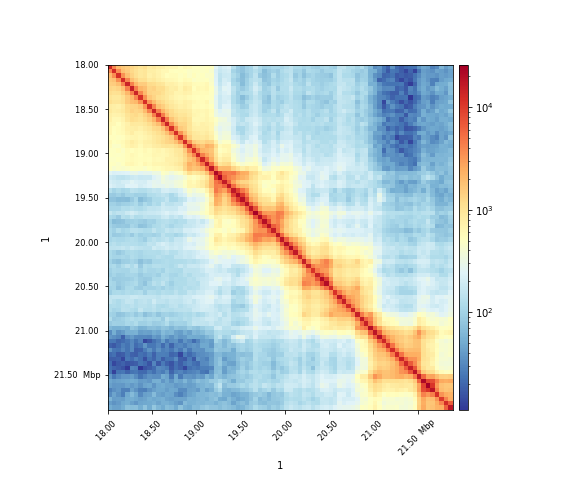
\includegraphics[scale=0.4]{figures/results/c_50kb}}
        \subfloat[RUST]{
            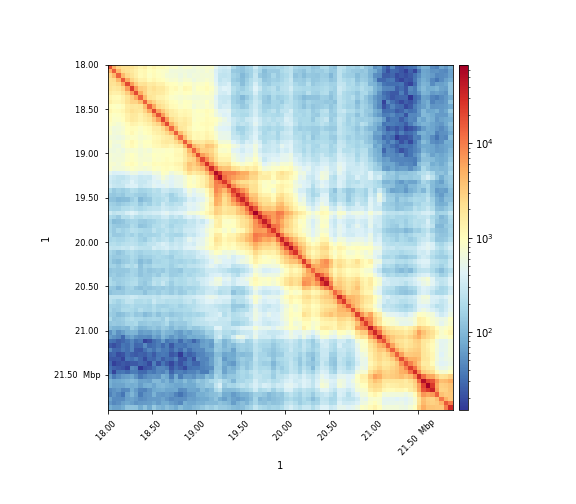
\includegraphics[scale=0.4]{figures/results/c_rust_50kb}} \\
        \subfloat[ICE]{
            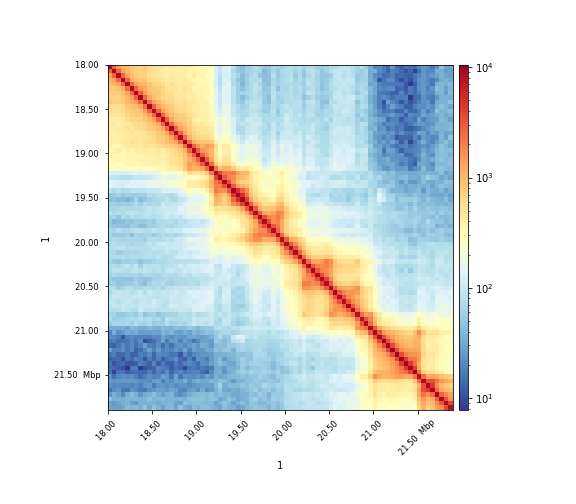
\includegraphics[scale=0.4]{figures/results/c_ice_50kb}}
        \subfloat[KR]{
            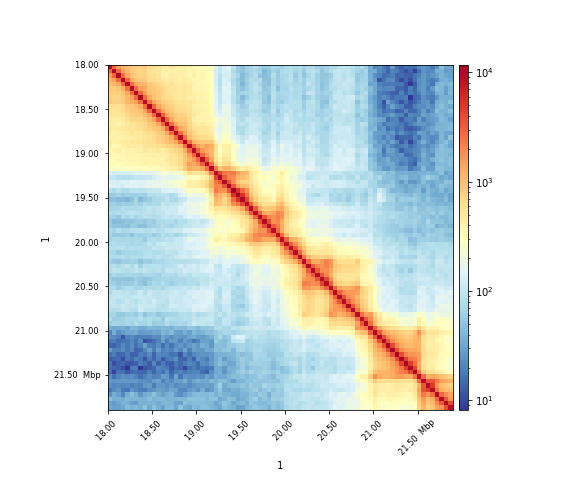
\includegraphics[scale=0.4]{figures/results/c_kr_50kb}}
        \caption[Plotting corrected matrices]
        {\textbf{Original and corrected matrices.} In \textbf{(b)} there appear to be
        higher maximum values, setting the cutoff lower creates pictures
        indistinguishable to those from ICE or KR.
        Images were created using hicPlotMatrix.
        }
        \label{fig:plotted}
    \end{centering}
\end{figure}
